\documentclass{standalone}

\usepackage{tikz}

\begin{document}
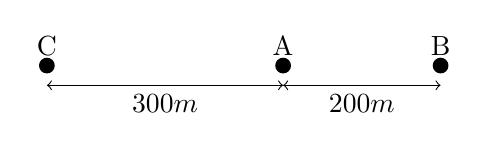
\begin{tikzpicture}

	\coordinate (A) at (3, 0);
	\coordinate (Ab) at (3, -0.25);
	\coordinate (B) at (5, 0);
	\coordinate (Bb) at (5, -0.25);
	\coordinate (C) at (0, 0);
	\coordinate (Cb) at (0, -0.25);

	\node[above] at (A) {A};
	\node[above] at (B) {B};
	\node[above] at (C) {C};

	\fill[black] (A) circle(0.1);
	\fill[black] (B) circle(0.1);
	\fill[black] (C) circle(0.1);

	\draw[<->] (Ab) -- (Bb) node[midway, below] {$200m$};
	\draw[<->] (Cb) -- (Ab) node[midway, below] {$300m$};

\end{tikzpicture}
\end{document}
